
\documentclass[11pt]{article}
\usepackage[utf8]{inputenc}
\usepackage[english]{babel}
\usepackage{amsthm, amsmath}
\usepackage{nccmath} %Para centrar ecuaciones
\usepackage{graphicx}
\usepackage{enumitem}
\graphicspath{ {Images/} }
    \title{\textbf{Práctica 1}}
    \author{Jorge Barceló Orellana}
    \date{}
    
    \addtolength{\topmargin}{-3cm}
    \addtolength{\textheight}{3cm}
\begin{document}

\maketitle
\thispagestyle{empty}

\section*{Ejercicio 1}
Find the power set R³
of R = \{(1, 1),(1, 2),(2, 3),(3, 4)\}. Check your answer with the script powerrelation.m and write a {\LaTeX} document with the
solution step by step.


\begin{equation}
	R =
	\begin{pmatrix}
	1 & 1 & 0 & 0\\
	0 & 0 & 1 & 0\\
	0 & 0 & 0 & 0\\
	0 & 0 & 0 & 0 
	\end{pmatrix}
\end{equation}

\begin{equation}
	R^2 = R \times R = 
	\begin{pmatrix}
	1 & 1 & 0 & 0\\
	0 & 0 & 1 & 0\\
	0 & 0 & 0 & 0\\
	0 & 0 & 0 & 0 
	\end{pmatrix}
	\times
	\begin{pmatrix}
	1 & 1 & 0 & 0\\
	0 & 0 & 1 & 0\\
	0 & 0 & 0 & 0\\
	0 & 0 & 0 & 0 
	\end{pmatrix}
	=
	\begin{pmatrix}
	1 & 1 & 1 & 0\\
	0 & 0 & 0 & 1\\
	0 & 0 & 0 & 0\\
	0 & 0 & 0 & 0 
	\end{pmatrix}
\end{equation}

\begin{equation}
	R^3 = R^2 \times R = 
	\begin{pmatrix}
	1 & 1 & 1 & 0\\
	0 & 0 & 0 & 1\\
	0 & 0 & 0 & 0\\
	0 & 0 & 0 & 0 
	\end{pmatrix}
	\times
	\begin{pmatrix}
	1 & 1 & 0 & 0\\
	0 & 0 & 1 & 0\\
	0 & 0 & 0 & 0\\
	0 & 0 & 0 & 0 
	\end{pmatrix}
	=
	\begin{pmatrix}
	1 & 1 & 1 & 1\\
	0 & 0 & 0 & 0\\
	0 & 0 & 0 & 0\\
	0 & 0 & 0 & 0 
	\end{pmatrix}
\end{equation}

\begin{equation}
	R^3 = \{(1,1),(1,2),(1,3),(1,4)\}
\end{equation}
\\
Comprobación con Octave:\\

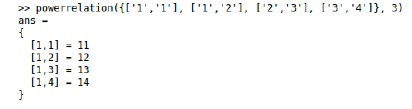
\includegraphics[scale=0.80]{ComprobacionOctave.PNG}


\end{document}

